\section{Visualizing Sparse Pathways}
As mentioned in section \ref{subsec:CustomLayer}, the MaxOut and ChannelOut layers applied in this 
analysis were created by me using the TensorFlow \ac{API}'s. As such, I found it imperative to make
sure that the layers worked as intended. To do this I created a small network with three layers, with 8 
nodes each, all applying MaxOut layers with 4, 2 and 4 groups respectively. In this section I will 
dissect the activations of said network before and after training.
\\
In figure \ref{fig:BTraining}, I have plotted the activation of 500
\begin{figure}
    \makebox[\linewidth][c]{%
    \centering
    \begin{subfigure}{.8\textwidth}
        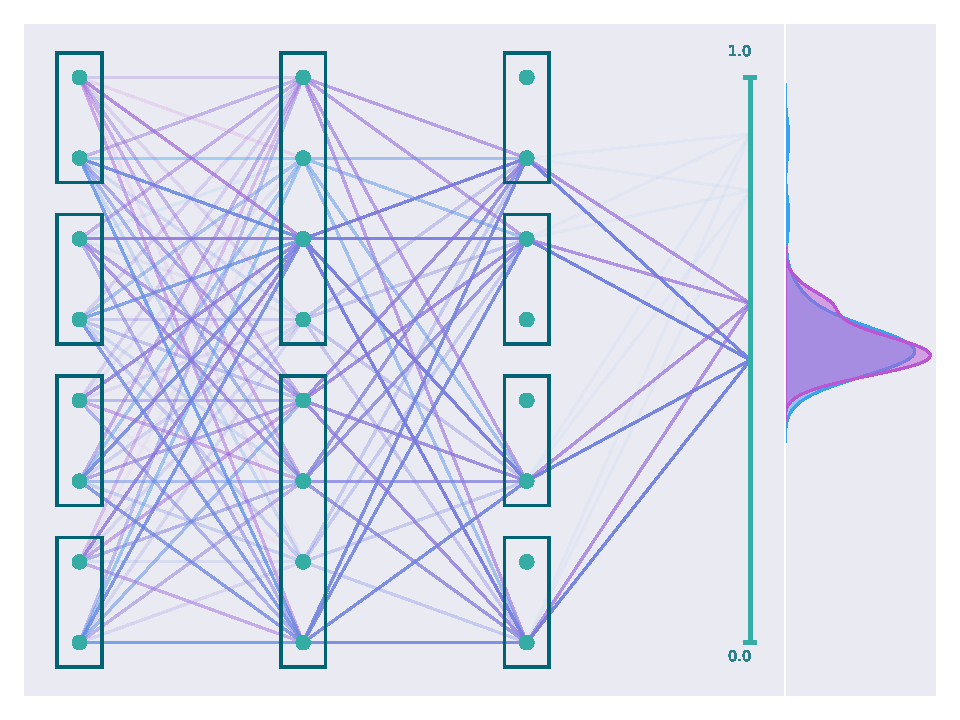
\includegraphics[width=\textwidth]{Figures/MLResults/NN/NetworkVis/BeforeTraining.pdf}
    \end{subfigure}
    }
    \caption{A calculated visualization of a 3 layer MaxOut network. Each line represents a 
    }
    \label{fig:BTraining}
\end{figure}
\begin{figure}
    \makebox[\linewidth][c]{%
    \centering
    \begin{subfigure}{.8\textwidth}
        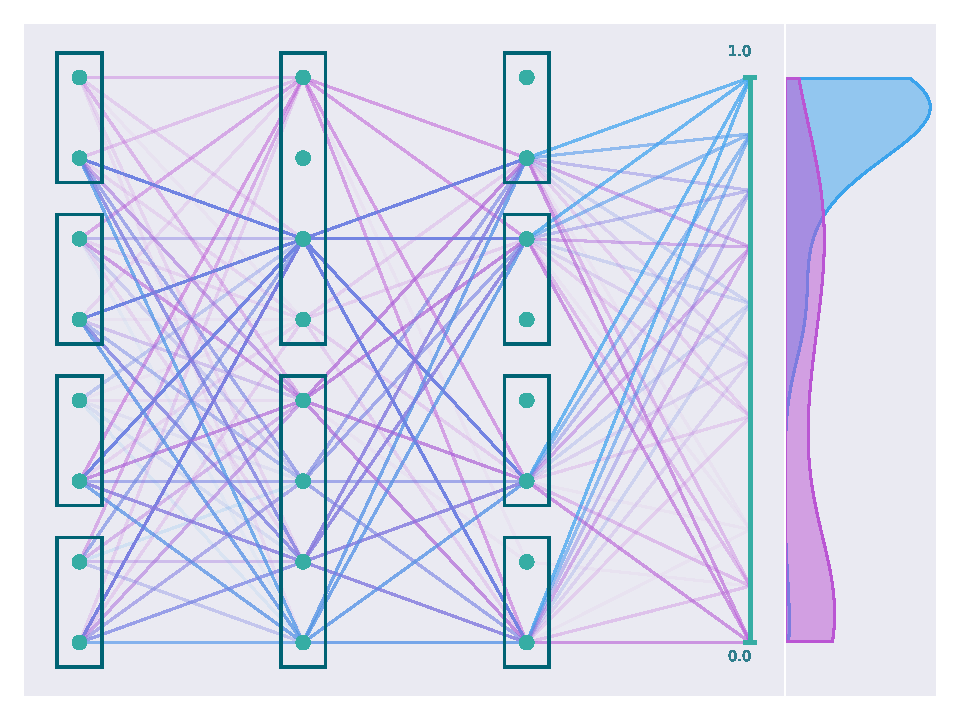
\includegraphics[width=\textwidth]{Figures/MLResults/NN/NetworkVis/AfterTraining.pdf}
    \end{subfigure}
    }
    \caption{The event distribution for each channel over the number of b-jets 
    with $77\%$ \ref{fig:nbjet77} and $85\%$ \ref{fig:nbjet85} efficiency.}
    \label{fig:ATraining}
\end{figure}

\begin{figure}
    \makebox[\linewidth][c]{%
    \centering
    \begin{subfigure}{.6\textwidth}
        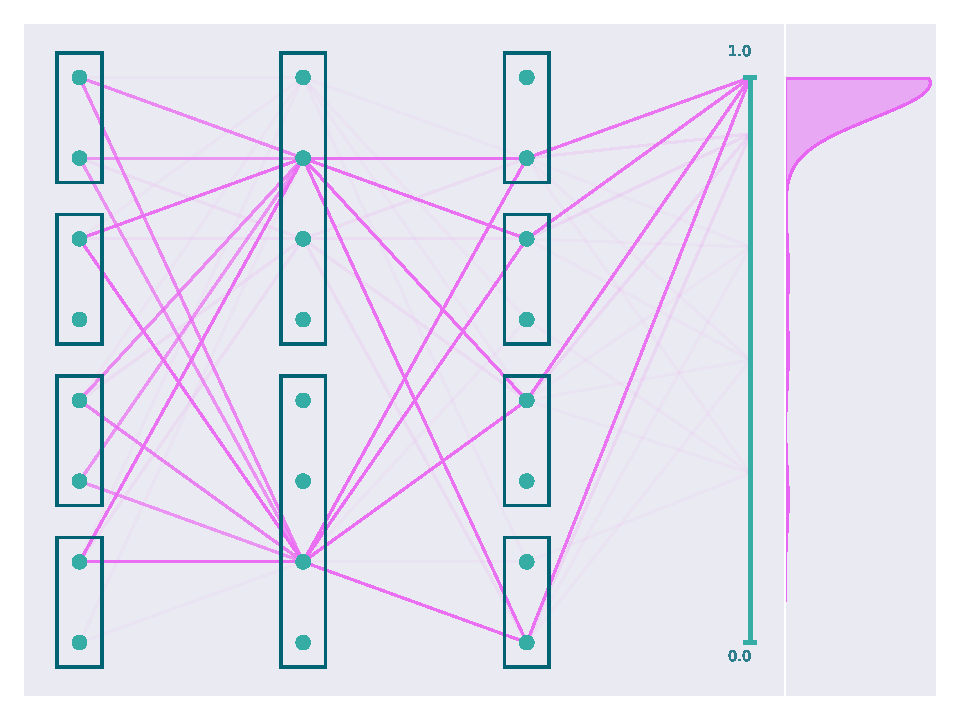
\includegraphics[width=\textwidth]{Figures/MLResults/NN/NetworkVis/AfterTrainingSig.pdf}
        \caption{}
        \label{fig:ATrainingSig}
    \end{subfigure}
    \hfill
    \begin{subfigure}{.6\textwidth}
        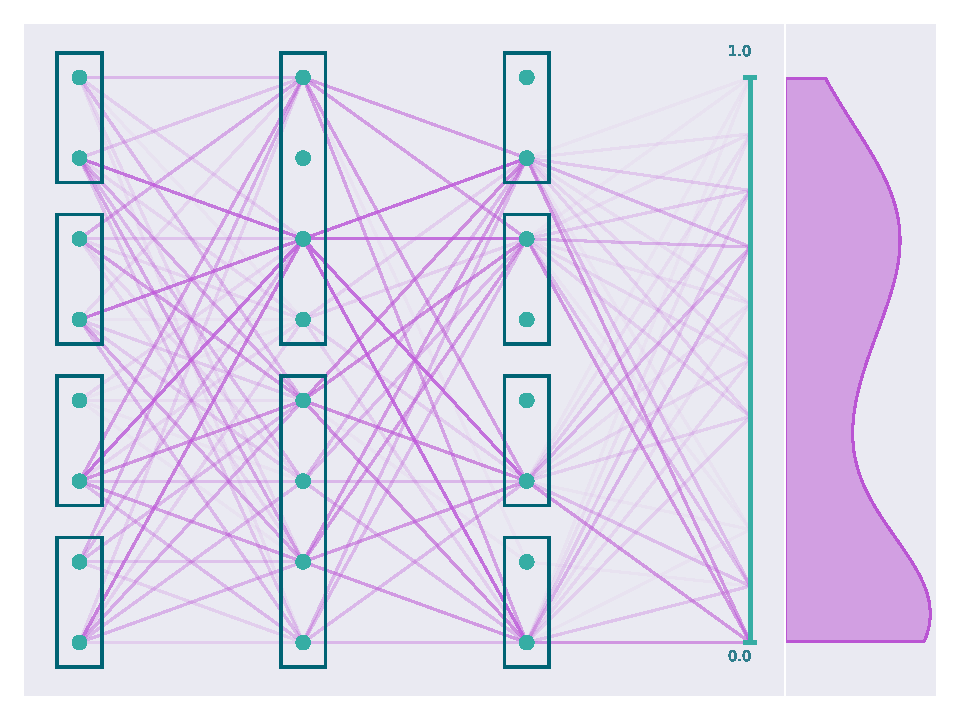
\includegraphics[width=\textwidth]{Figures/MLResults/NN/NetworkVis/AfterTrainingBkg.pdf}
        \caption{}
        \label{fig:ATrainingBkg}
    \end{subfigure}
    }
    \caption{The event distribution for each channel over the number of b-jets 
    with $77\%$ \ref{fig:nbjet77} and $85\%$ \ref{fig:nbjet85} efficiency.}
    \label{fig:NetDist}
\end{figure}